\documentclass[11pt]{article}
\usepackage[margin=1in]{geometry}
\usepackage{amsmath,amssymb}
\usepackage{booktabs}
\usepackage{enumitem}
\usepackage{pgfplots}
\pgfplotsset{compat=1.17}
\usepgfplotslibrary{groupplots}
\usepackage[hidelinks]{hyperref}

\title{\textbf{ContainmentBench: A Benchmark for Mitigation Policies on
Competing-Diffusion (Chase--Escape) Processes}}
\author{Archit Sharma\thanks{Project Lifeline. \texttt{archit.sharma@nometria.com}.
Code: \url{https://github.com/matrix-share/matrix} (\texttt{benchmarks/containment}).}}
\date{\today}

\newcommand{\Nwin}{N_{\mathrm{win}}}
\newcommand{\rhoc}{\rho^\star}

\begin{document}
\maketitle

\begin{abstract}
Many security and social systems face the same problem: a harmful thing spreads
through a network while a detection/mitigation process chases it, and the question
is how much harm accrues before it is contained. Examples include offline
double-spending of a bearer capability chased by gossiped revocation, and a rumour
chased by fact-checks. This is the \emph{chase-escape} (predator--prey) percolation
process. We present \textbf{ContainmentBench}, a reproducible, pip-installable
benchmark that turns this process into a control problem: an agent observes a
spreading over-spend front and allocates a budget of detection effort to minimize
the harm at low cost. The benchmark ships (i)~a fast pure-Python environment
validated against a Rust reference implementation; (ii)~a task suite spanning
well-mixed, 2-D lattice, random-geometric (RGG), and Random-Waypoint mobility
topologies; (iii)~cost-normalized metrics and a policy interface; and (iv)~a
baseline leaderboard. As reference findings we confirm the mean-field
$\mathbb{E}[\Nwin]\!\sim\!(a/d)\ln N$ over-spend law, the well-mixed$\to$spatial
containment dichotomy, and---extending prior lattice-only analysis---a
\emph{topology-dependent} critical ratio $\rhoc$ (lattice $\approx0.47$, RGG
$\approx0.78$, mobility $<0.30$), identifying realistic mobility as the hardest
case. Baselines reveal that the best policy is topology-dependent and that a simple
front-reactive heuristic is Pareto-better than always-on detection, leaving clear
headroom for learned policies. Everything is seeded and open.
\end{abstract}

\section{Introduction}
A recurring pattern across security and networked social systems is a race between
two spreading processes: something harmful propagates (an over-spent offline token,
a rumour, a worm) while a mitigation process (gossiped revocation, fact-checking,
patching) propagates to stop it. The realized harm---how many nodes the harmful
process reaches before mitigation catches it---depends on the \emph{ratio} of the
two speeds and on the \emph{topology} they race over. This is exactly the
\emph{chase-escape} process studied in probability~\cite{chaseescape}, and the
applied question ``how much harm, and can we contain it under a mitigation budget?''
is a control problem that, to our knowledge, lacks a standard benchmark.

We provide one. ContainmentBench frames containment as a sequential decision problem
over the chase-escape dynamics and supplies the environment, tasks, metrics,
baselines, and a leaderboard, in the mold of recent benchmark contributions whose
value is a reproducible environment plus an empirical finding rather than a new
theorem~\cite{real}. Our motivation is concrete: in an offline mesh messenger, a
metered gateway capability is a bearer token that can be over-spent across a
partition, and gossiped revocation is the only thing that contains
it~\cite{containment}; the same mathematics governs misinformation
containment~\cite{chaseescape}.

\paragraph{Contributions.}
\begin{enumerate}[leftmargin=1.4em,itemsep=1pt]
  \item \textbf{An environment + benchmark} for containment/mitigation policies on
  chase-escape processes: a pure-numpy, Gymnasium-style env validated against a Rust
  reference, with tasks over four topologies, cost-normalized metrics, and a policy API.
  \item \textbf{Reference findings} shipped with the benchmark: the mean-field
  $\ln N$ over-spend law; the well-mixed$\to$spatial containment dichotomy; and a
  \emph{topology-dependent} critical ratio $\rhoc$ that extends prior lattice-only
  results to RGG and mobility, singling out realistic mobility as the hardest regime.
  \item \textbf{A baseline leaderboard} showing the best policy is topology-dependent,
  a front-reactive heuristic Pareto-dominates always-on detection, and no baseline
  contains the mobility case---quantified headroom for learned policies.
\end{enumerate}

\section{The containment process}
A graph $G=(V,E)$ carries three node states: White (susceptible), Red (harmed /
over-spent), Blue (mitigated). Red nodes fire at rate $\lambda_r$, converting a
random White neighbour to Red (the harm spreads). Blue nodes fire at rate
$\lambda_b$, converting a random Red neighbour to Blue (mitigation catches harm and
rides its trail). The order parameter is the realized harm $\Nwin=\#\{\text{nodes
ever Red}\}$; the control ratio is $\rho=\lambda_r/\lambda_b$. There is also a
\emph{non-transferable} special case (a single harmful agent rather than a spreading
one) whose mean-field over-spend is $\mathbb{E}[\Nwin]=\sum_{j}a/(a+dj)\sim(a/d)\ln
N$~\cite{containment}. A \emph{policy} sets the mitigation rate $\lambda_b$ over time
(and, in richer variants, space) from partial observations of the front, under a
cost that is the detection effort spent.

\section{ContainmentBench}
\paragraph{Environment.} \texttt{ContainmentEnv} advances the process in chunks of
micro-events; each step the agent picks a discrete detection level mapped to
$\lambda_b\in[0,\lambda_b^{\max}]$. Observation: $[\text{red frac},\text{blue
frac},\text{over-spent frac},\text{front frac},t/H]$. Reward: $-(\text{new
over-spends})/N-\lambda\cdot(\text{detection intensity})$. Episodes end on
containment (prey extinct), horizon, or budget exhaustion. The dynamics are pure
numpy; a Rust implementation (\texttt{crates/sim}) is the reference, and
\texttt{validate.py} checks the numpy port reproduces it (the $\ln N$ ratio and
$\rhoc$) within noise.

\paragraph{Topologies.} \emph{well-mixed} (complete graph, mean-field), \emph{2-D
torus lattice} (the reference spatial case), \emph{random-geometric graph} (RGG; the
standard wireless-mesh model), and a \emph{Random-Waypoint} mobility snapshot (RGG on
positions drawn from the RWP stationary density, which concentrates nodes centrally).
RGG and mobility are new relative to prior lattice-only analysis.

\paragraph{Metrics.} over-spent fraction $\Nwin/N$; detection intensity
$\in[0,1]$ (average $\lambda_b/\lambda_b^{\max}$ actually spent); the cost-normalized
objective $\Nwin/N+\lambda\cdot\text{intensity}$ (lower is better); runaway
probability (order parameter); and containment AUC over a $\rho$ sweep.

\section{Reference findings}
These ship with the benchmark as validated ``ground truth''; all are reproducible
from \texttt{crates/sim} and \texttt{benchmarks/containment}.

\paragraph{(1) The mean-field $\ln N$ law (Fig.~\ref{fig:lnn}).} For the
non-transferable agent with $a=d=1$, $\mathbb{E}[\Nwin]/\ln N$ is flat at
${\approx}1.09=a/d$ across four decades of $N$: harm grows, but only logarithmically.

\paragraph{(2, 3) Dichotomy and a topology-dependent $\rhoc$ (Fig.~\ref{fig:topo}).}
On a well-mixed graph, trail-confined mitigation runs away at \emph{every} $\rho$ (a
single mitigation seed, diluted $1/N$, cannot catch an exponentially spreading harm).
On every \emph{spatial} topology it contains below a finite critical ratio---but that
ratio is topology-dependent: lattice $\rhoc\!\approx\!0.47$ (matching the known planar
chase-escape point), uniform RGG $\rhoc\!\approx\!0.78$ (\emph{easier} to contain),
and Random-Waypoint mobility $\rhoc\!<\!0.30$ (\emph{harder}: its central node-density
creates high-degree hubs that accelerate spread). Realistic mobility is thus the
hardest regime---exactly the case prior lattice-only analysis left open.

\begin{figure}[t]\centering
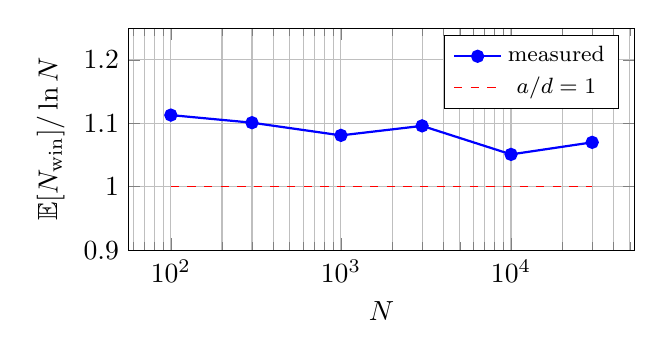
\begin{tikzpicture}
\begin{axis}[width=.66\linewidth,height=4.4cm,xmode=log,log basis x=10,
  xlabel={$N$},ylabel={$\mathbb{E}[\Nwin]/\ln N$},ymin=0.9,ymax=1.25,grid=both,
  legend pos=north east,legend style={font=\footnotesize}]
\addplot[thick,mark=*,blue] coordinates
 {(100,1.113)(300,1.101)(1000,1.081)(3000,1.096)(10000,1.051)(30000,1.070)};
\addplot[dashed,red,no marks] coordinates {(100,1.0)(30000,1.0)};
\legend{measured,$a/d=1$}
\end{axis}
\end{tikzpicture}
\caption{Reference finding 1: the mean-field over-spend law $\mathbb{E}[\Nwin]\sim
(a/d)\ln N$ (ratio flat across four decades).}\label{fig:lnn}
\end{figure}

\begin{figure}[t]\centering
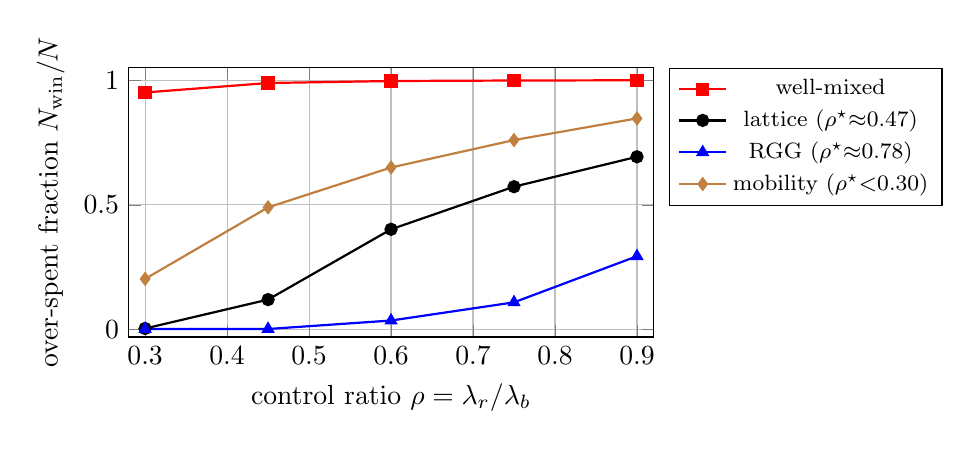
\begin{tikzpicture}
\begin{axis}[width=.68\linewidth,height=5cm,xlabel={control ratio $\rho=\lambda_r/\lambda_b$},
  ylabel={over-spent fraction $\Nwin/N$},xmin=0.28,xmax=0.92,ymin=-0.03,ymax=1.05,
  grid=both,legend pos=outer north east,legend style={font=\footnotesize}]
\addplot[thick,mark=square*,red] coordinates {(0.30,0.951)(0.45,0.989)(0.60,0.997)(0.75,0.999)(0.90,1.000)};
\addplot[thick,mark=*,black] coordinates {(0.30,0.004)(0.45,0.120)(0.60,0.402)(0.75,0.573)(0.90,0.693)};
\addplot[thick,mark=triangle*,blue] coordinates {(0.30,0.002)(0.45,0.002)(0.60,0.036)(0.75,0.109)(0.90,0.294)};
\addplot[thick,mark=diamond*,brown] coordinates {(0.30,0.203)(0.45,0.490)(0.60,0.650)(0.75,0.760)(0.90,0.847)};
\legend{well-mixed,lattice ($\rhoc{\approx}0.47$),RGG ($\rhoc{\approx}0.78$),mobility ($\rhoc{<}0.30$)}
\end{axis}
\end{tikzpicture}
\caption{Reference findings 2--3: well-mixed mitigation runs away at every $\rho$;
all spatial topologies contain below a \emph{topology-dependent} critical ratio
$\rhoc$. Uniform RGG is easiest to contain, Random-Waypoint mobility hardest.}
\label{fig:topo}
\end{figure}

\section{Baseline leaderboard}
Table~\ref{tab:lb} scores baseline policies on three tasks (one per spatial
topology, adversary rate $\lambda_r=0.6$ in the containable regime, $\lambda=0.3$),
averaged over graph$\times$seed replicas. Findings: (i)~the best policy is
\emph{topology-dependent}---a front-reactive heuristic wins on the lattice, cheap
constant detection suffices on easy RGG, and only maximal detection helps on hard
mobility; (ii)~\texttt{reactive-front} matches always-on containment at lower cost
(Pareto-better); (iii)~\emph{no baseline contains the mobility task} (best over-spent
$0.159$), quantifying the headroom a learned policy (a companion RL track) can target.

\begin{table}[t]\centering\small
\caption{Baseline leaderboard. Objective $=$ over-spent fraction $+\,\lambda\cdot$
detection intensity ($\lambda=0.3$; lower is better). Best per task in \textbf{bold}.}
\label{tab:lb}
\begin{tabular}{@{}l ccc c ccc c ccc@{}}
\toprule
& \multicolumn{3}{c}{\textbf{lattice}} && \multicolumn{3}{c}{\textbf{RGG}} && \multicolumn{3}{c}{\textbf{mobility}}\\
\cmidrule{2-4}\cmidrule{6-8}\cmidrule{10-12}
policy & o.s. & cost & obj && o.s. & cost & obj && o.s. & cost & obj\\
\midrule
no-detect      & .418 & .00 & .418 && .368 & .00 & .368 && .573 & .00 & .573\\
constant-0.5   & .262 & .50 & .412 && .087 & .50 & \textbf{.237} && .431 & .50 & .581\\
fixed-rate     & .262 & .50 & .412 && .087 & .50 & \textbf{.237} && .431 & .50 & .581\\
max-detect     & .012 & 1.0 & .312 && .010 & 1.0 & .310 && .159 & 1.0 & \textbf{.459}\\
reactive-front & .012 & .92 & \textbf{.289} && .011 & .81 & .253 && .159 & 1.0 & \textbf{.459}\\
random         & .382 & .54 & .543 && .240 & .57 & .410 && .571 & .50 & .721\\
\bottomrule
\end{tabular}
\end{table}

\section{Related work}
Chase-escape and competing first-passage percolation are studied in
probability~\cite{chaseescape}; our applied framing and the security instance are
from~\cite{containment}. Benchmarks whose contribution is a reproducible environment
plus an empirical finding are now common in ML~\cite{real}. Learning to intervene on
diffusion (epidemic control, influence, misinformation) is active; ContainmentBench
offers a controlled, seeded testbed with a measured critical structure.

\section{Limitations and intended use}
The dynamics are an abstract model, not a packet-level simulator; the mobility model
is a stationary snapshot; and the baseline suite is deliberately simple (its purpose
is to establish headroom, not to be strong). $\rhoc$ estimates use a modest
finite-size study---precise exponents need larger runs. The benchmark is intended for
research on containment/mitigation policies and diffusion intervention, not as a
deployable fraud system.

\section{Reproducibility}
Pure numpy; \texttt{pip install -e benchmarks/containment}; \texttt{python -m
containment\_bench.validate} reproduces the reference facts; \texttt{run\_reference}
and \texttt{run\_benchmark} regenerate the figures and Table~\ref{tab:lb}. All runs
are seeded; CSVs are committed under \texttt{docs/research/data} and
\texttt{benchmarks/containment/results}.

\begin{thebibliography}{9}
\bibitem{containment} A.~Sharma. \emph{Containing an Adversarial Bearer Token in a
Partitionable Mesh}. Project Lifeline research note, 2026.
\bibitem{chaseescape} R.~Durrett, M.~Junge, S.~Tang. \emph{Coexistence in
chase-escape}. Electron.\ Commun.\ Probab., 2020; and works on competing
first-passage percolation.
\bibitem{real} D.~Garg et al. \emph{REAL: Benchmarking Autonomous Agents on
Deterministic Simulations of Real Websites}. NeurIPS Datasets \& Benchmarks, 2025.
\end{thebibliography}

\end{document}
